\documentclass{report}

\usepackage{subcaption} % package for subfigures
\usepackage{hyperref}  % package for linking figures etc
\usepackage{enumitem}  % package for description with bullets
\usepackage{graphicx}  % package for importing images
\usepackage{mathtools} % package for math equation
\usepackage{mathrsfs}  % package for math font
\usepackage{indentfirst} % package for getting ident after section or paragraph
\usepackage{multirow}  % package for tables, multirow
\usepackage{longtable} % package for multi pages tables


\usepackage[export]{adjustbox}
% \usepackage{amsmath}

\setlength{\parindent}{2em} % how much indent to use when we start a paragraph

\graphicspath{ {./theory/figures/} }       % path for images

\begin{document}

\chapter{Connecting Tubes}
\section{Description}
After getting TOIs for each video segment, it is time to connect them. That's because most actions in videos lasts more that 16 frames.
This means that, in overlaping video clips, there will be consequentive TOIs that represent the entire action. So, it is essential to create
an algorithm for finding and connecting these TOIs.

\section{First approach: combine overlap and actioness}
Our algorithm is inspired by \cite{DBLP:journals/corr/HouCS17}, which calculates all possible sequences of ToIs. In order find the best candidates,
it uses a score which tells us how likely a sequence of TOIs is  to contain an action. This score is a combination of 2 metrics:
\begin{description}
\item[ Actioness,  ] which is the TOI's possibility to contain an action. This score is produced by TPN's scoring layers.
\item [ TOIs' overlapping, ] which is the IoU of the last frames of the first TOI and the first frames of the second TOI.
\end{description}

The above scoring policy can be described by the following formula:
\[ S = \frac{1}{m} \sum_ {i=1}^{m} Actioness_i + \frac{1}{m-1} \sum_{j=1}^{m-1} Overlap_{j,j+1} \]

For every possible combination of TOIs we calculate their score as show in figure \ref{fig:connection_algo}.

\begin{figure}[h]
  \centering
  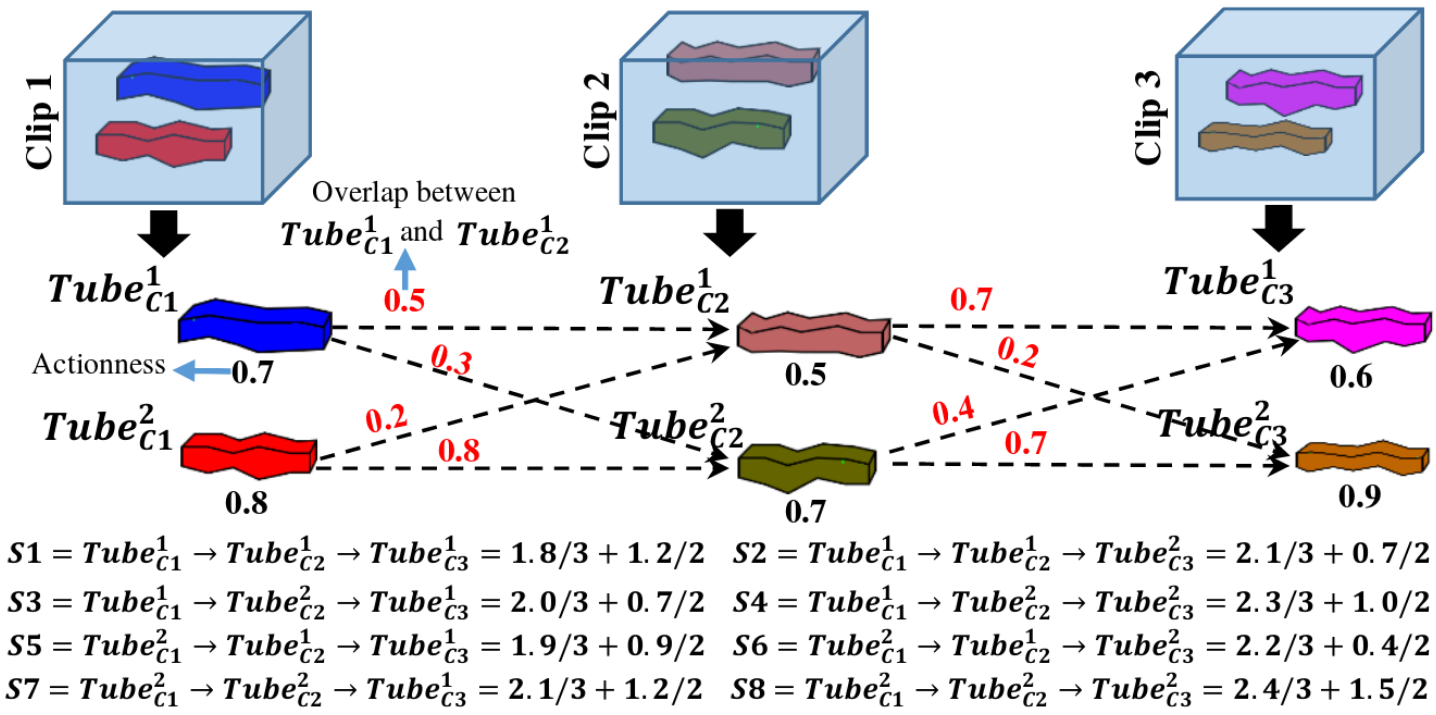
\includegraphics[scale=0.225]{connection_algo}
  \caption{An example of calculating connection score for 3 random TOIs}
  \label{fig:connection_algo}
\end{figure}

The above approach, however, needs too much memory for all needed calculations, so a memory usage  problem is
appeared. The reason is, for every new video segments we propose \textit{k TOIs} (16 during training and 150 during validation).
As a result, for a small video seperated in  \textbf{10 segments}, we need to calculate 
\textbf{  150\textsuperscript{10} scores} during validation stage. This causes our system to overload and it takes too much time to process
just one video. \par

In order to deal with this problem, we create a greedy algorithm in order to find the candidates tubes. Inituitively, this algorithm after
a new video segment keeps tubes with score higher than a threshold, and deletes the rest. So, we don't need to calculate combinations with
very low score. We wrote code for calculating tubes' scores in CUDA language, which has the ability to
parallel process the same code using different data. Our algorithm is described below:

\begin{enumerate}
\item Firstly,  initialize empty lists for the final tubes, final tubes' duratio, their scores, active tubes, their correnspondig duration,
  active tubes' overlapping sum and actioness sum where:
  \begin{itemize}
  \item Final tubes list contains all tubes which are the most likely to contain an action, and their score list contains their
    corresponding scores. We refer to each tube by its index which is related a tensor, in which we saved all the ToIs proposed
    from TPN for each video segment.
  \item Active tubes list contains all tubes that will be match with the new TOIs. Their overlapping sum list and actioness sum list
    contain their sums in order to avoid calculating then for each loop. 
  \end{itemize}
Also, we initialize threshold equal to 0.5 .
\item For the first video segment, we add all the TOIs to both active tubes and final tubes. Their scores are only their actioness because
  there are no tubes for calculating their overlapping score. So, we set their overlaping sum equal to 0.
\item For each next video, after getting the proposed ToIs, firstly we calculate their overlapping score with each active tube. Then, we
  empty active tubes, active tubes' duration, overlapping sum and actioness score lists.  For each new tube that has score higher than the threshold
  we add both to final tubes and to active tubes, and we increase their duration.
\item If the number of active tubes is higher than a threshold, we set the threshold equal to the score of
  the 100th higher score. On top of that, we update the final tubes list, removing all tubes that have score lower than the threshold.
\item After that, we add in active tubes, the current video segment's proposed TOIs. Also their actioness scores in actioness sum list and
  zero values in corrensponding positions in overlaps sum list (such as in the 1st step).
\item We repeat the previous 3 steps until there is no video segment left.
\item Finally, as we mentioned before, we have a list which contains the indexes of the saved tubes. So, we modify them in order to have
  the final bounding boxes. However, 2 succeeding ToIs do not have extactly the same bounding boxes in the frames that overlap. For example,
  ToIs from the $1^{st}$ video segment start from frame 1 to frame 16. If we have video step equal with 8, it overlaps with the ToIs from the
  succeeding video segment in frames 8-16. In those frames, in final tube, we choose the area that contains both bounding boxes which is
  denoted as $(min(x_1,x'_1), min(y_1,y'_1), max(x_2,x'_2), max(y_2,y'_2))$ for bounding boxes $(x_1,y_1,x_2,y_2)$ and $(x'_1,y'_1,x'_2,y'_2)$.
\end{enumerate}
% We implement this algorithm using CUDA language for counting the scores. In \cite{DBLP:journals/corr/HouCS17}, they use temporal \textit{stride = sample duration} during testing. We want 
\subsection{JHMDB Dataset}

In order to validate our algorithm, we firstly experiment in JHMDB dataset's videos in order to define the best overlapping policy and
the video overlapping step. Again, we use recall as evaluation metrinc. A groundtruth action tube is considered to be found, as well as positive,
if there is at least 1 video tube which overlaps with it over a predefined threshold, otherwise it .  These thresholds are again 0.5, 0.4 and 0.3.
We set TPN to return 30 ToIs per video segment.
We chose to update threshold when active tubes are more than 500 and to keep the first 100 tubes as active. We did so, because, a big part of the
code is performing in CPU. That's because, we use lists, which are very easy to handle for adding and removing elements. So, if we use bigger update
limits, it takes much more time to process them.

\paragraph{sample duration = 16} At first we use as sample duration = 16 and video step = 8. As overlapping frames we count frames
\textit{(8...15)} so we have \#8 frames. Also, we use only \#4 frames with combinations \textit{(8...11), (10...13) and (12...15)} and 
\#2 frames with combinations \textit{(8,9), (10,11), (12,13), and (14,15)}. The results are shown in Table \ref{table:step8_16} (in bold are
the frames with which we calculate the overlap score).

\begin{center}
\begin{longtable}{||c||c c c||}

  \hline
  \multirow{2}{5em}{combination} & {} &overlap thresh & {} \\
                                    &  0.5  &  0.4 &  0.3 \\         
  \hline  \hline
  0,1,...,\textbf{\{8,...,15\}}               & {} & {} & {} \\
  \textbf{\{8,9,...,15\}},16,...,23           & 0.3172 & 0.4142 & 0.6418 \\
  \hline     \hline                          


  0,1,...,\textbf{\{8,...,11,\}}...,14,15     & {} & {} & {} \\
  \textbf{\{8,...,11\}},12,...,22,23          & 0.3172 & 0.4142& 0.6381 \\
  \hline
  0,1,...,\textbf{\{10,...,13,\}}14,15,       & {} & {} & {} \\
  8,9,\textbf{\{10,...,13\}},14,...,22,23     & 0.3209 &0.4179   & 0.6418 \\
  \hline
  0,1,...,\textbf{\{12,...,15,\}}             & {} & {} & {} \\
  8,9,...,\textbf{\{12,...,15\}},16,...,23,   & 0.3284 & 0.4216 & 0.6381 \\
  \hline     \hline                          

  0,1,...,\textbf{\{8,...,11,\}},...,14,15,   & {} & {} & {} \\
  \textbf{\{8,9,...,11,\}}12,...,22,23        & 0.3172   & 0.4142& 0.6381 \\
  \hline
  0,1,...,\textbf{\{10,...,13,\}}14,15,       & {} & {} & {} \\
  \textbf{\{10,...,13\}},14,...,22,23         & 0.3209 &0.4179   & 0.6418 \\
  \hline
  0,1,...,\textbf{\{12,...,15\}}              & {} & {} & {} \\
  8,9,...,\textbf{\{12,...,15\}},16,...       & 0.3284 & 0.4216 & 0.6381 \\
  \hline \hline
  
  0,1,...,\textbf{\{8,9,\}},10,...,14,15,     & {} & {} & {} \\
  \textbf{\{8,9,\}}10,11,...,22,23            & 0.3134   & 0.4104 & 0.6381 \\
  \hline
  0,1,...,\textbf{\{10,11,\}},12,...,14,15,   & {} & {} & {} \\
  8,9,\textbf{\{10,11,\}}12,...,22,23         & 0.3209   & 0.4216 & 0.6418 \\
  \hline
  0,1,...,\textbf{\{12,13,\}},14,15,          & {} & {} & {} \\
  8,9,...,\textbf{\{12,13,\}}14,...,22,23     & 0.3246   & 0.4179 & 0.6418 \\
  \hline
  0,1,...,13,\textbf{\{14,15,\}}              & {} & {} & {} \\
  8,9,...,\textbf{\{14,15,\}}16,...,22,23     & 0.3321   & 0.4216 & 0.6306 \\
  \hline \hline
  \caption{Recall results for step = 8}
  \label{table:step8_16}
\end{longtable} 
\end{center}

As we can from the above table, generally we get very bad performance and we got the best performance when we calculate the overlap between only 2 frames (either \textit{14,15} or \textit{12,13}).
So, we thought that we should increase the video step because, probably, the connection algorithm is too strict into big movement variations during  the video. As a results, we set video step = 12 which
means that we have only 4 frames overlap. In this case,  for \#4 frames, we only have the combination \textit{(12...15)}, for \#2 frames we have \textit{(12,13), (13,14) and (14,15)} as shown in
Table \ref{table:step12_16}.

\begin{center}
\begin{longtable}{||c||c c c||}

  \hline
  \multirow{2}{5em}{combination} & {} &overlap thresh & {} \\
                                    &  0.5  &  0.4 &  0.3 \\         
  \hline  \hline
  0,1,...,11,\textbf{\{12,...,15\}}           & {} & {} & {} \\
  \textbf{\{12,13,...,15\}},16,...,26,27         & 0.3769 & 0.4627 & 0.6828 \\
  \hline     \hline                          

  0,1,...,\textbf{\{12,13,\}},14,15,          & {} & {} & {} \\
  \textbf{\{12,13,\}}14,15,...,26,27          & 0.3694   & 0.4627 & 0.6903 \\
  \hline                          
  0,1,...,12\textbf{\{13,14,\}},15,           & {} & {} & {} \\
  12,\textbf{\{13,14,\}}15,...,26,27          & 0.3843   & 0.4627 & 0.6828 \\
  \hline                          
  0,1,...,12,13\textbf{\{14,15,\}}            & {} & {} & {} \\
  12,13,\textbf{\{14,15,\}}16,...,26,27       & 0.3694   & 0.459 & 0.6828 \\
  \hline     \hline                          

  \caption{Recall results for step = 12}
  \label{table:step12_16}
\end{longtable} 
\end{center}

As we can see, recall performance is increase so that means that our assumption was correct. So again, we increase video step into 14, 15 and 16 frames
and recall score is shown at Table \ref{table:step14_16}
\begin{center}
\begin{longtable}{||c||c c c||}

  \hline
  \multirow{2}{5em}{combination} & {} &overlap thresh & {} \\
                                    &  0.5  &  0.4 &  0.3 \\         
  \hline  \hline
  0,1,...,13\textbf{\{14,15\}}                & {} & {} & {} \\
  \textbf{\{14,15\}},16,...,28,29                & 0.3731 & 0.5336 & 0.6493 \\
  \hline     \hline                          

  0,1,...,13,\textbf{\{14,\}}15,              & {} & {} & {} \\
  \textbf{\{14,\}}15,...,28,29                & 0.3694   & 0.5299 & 0.6455 \\
  \hline                          
  0,1,...,14,\textbf{\{15\}}                  & {} & {} & {} \\
  14,\textbf{\{15,\}}16,...,28,29             & 0.3731   & 0.5187 & 0.6381 \\
  \hline  \hline

  0,1,...,14,\textbf{\{15\}}                & {} & {} & {} \\
  \textbf{\{15\}},16,...,30                 & 0.3918 & 0.5187 & 0.6381 \\
  \hline     \hline                          
  0,1,...,14,\textbf{\{15\}}                & {} & {} & {} \\
  \textbf{\{16\}},17,...,31                 & 0.4067 & 0.7313 & 0.8731 \\
  \hline                          
  \caption{Recall results for steps = 14, 15 and 16}
  \label{table:step14_16}
\end{longtable} 
\end{center}

The results show that we get the best recall performance when we have no overlapping steps and video step = 16 = sample duration. We try to improve
more our results, using smaller duration because, as we saw from TPN recall performance, we get better results when we have sample duration = 8 or 4.

\paragraph{sample duration = 8}
We wanted to confirm that we get the best results, when we have no overlapping frames and step = sample duration. So Table \ref{table:step4_8}
shows recall performance for sample duration = 8 and video step = 4 and Table \ref{table:step8_678 } for video steps = 6, 7 and 8.


\begin{center}
\begin{longtable}{||c||c c c||}

  \hline
  \multirow{2}{5em}{combination} & {} &overlap thresh & {} \\
                                    &  0.5  &  0.4 &  0.3 \\         
  \hline  \hline
  0,1,2,3,13\textbf{\{4,5,6,7\}}                & {} & {} & {} \\
  \textbf{\{4,5,6,7\}},8,9,10,11                & 0.2015   & 0.3582 & 0.5858 \\
  \hline     \hline                          

  0,1,2,3,\textbf{\{4,5,\}}6,7                  & {} & {} & {} \\
  \textbf{\{4,5,\}}6,7,8,9,10,11                & 0.1978   & 0.3582 & 0.5933 \\
  \hline                          
  0,1,2,3,4\textbf{\{5,6,\}}7                   & {} & {} & {} \\
  4,\textbf{\{5,6,\}}7,8,9,10,11                & 0.1978   & 0.3507 & 0.5821 \\
  \hline                          
  0,1,2,3,4,5\textbf{\{6,7\}}                   & {} & {} & {} \\
  4,5,\textbf{\{6,7,\}}8,9,10,11                & 0.194   & 0.3433 & 0.585 \\
  \hline                           
  \caption{Recall results for step = 4}
  \label{table:step4_8}
\end{longtable} 
\end{center}

\begin{center}
\begin{longtable}{||c||c c c||}

  \hline
  \multirow{2}{5em}{combination} & {} &overlap thresh & {} \\
                                    &   0.5  &  0.4 &  0.3 \\         
  \hline  \hline
  0,1,2,3,4,5\textbf{\{6,7\}}           & {} & {} & {} \\
  \textbf{\{6,7\}},8,9,10,11,12,13      & 0.3134  & 0.7015 & 0.8619 \\
  \hline     \hline                          

  0,1,2,3,4,5,\textbf{\{6,\}}7          & {} & {} & {} \\
  \textbf{\{6,\}}7,8,9,10,11,12,13      & 0.3209  & 0.6679 & 0.847 \\
  \hline                          
  0,1,2,3,4,5,6,\textbf{\{7\}}          & {} & {} & {} \\
  6,\textbf{\{7\}}8,9,10,11,12,13       & 0.3172  & 0.6567 & 0.8507 \\
  \hline                          
  0,1,2,3,4,5,6\textbf{\{7\}}           & {} & {} & {} \\
  \textbf{\{7,\}}8,9,10,11,12,13,14     & 0.5597  & 0.7687 & 0.903 \\
  \hline                           
  0,1,2,3,4,5,6\textbf{\{7\}}           & {} & {} & {} \\
  \textbf{\{8\}}9,10,11,12,13,14,15     & 0.653	  & 0.8396 &0.9179  \\
  \hline                           
  \caption{Recall results for steps = 6, 7 and 8}
  \label{table:step8_678 }
\end{longtable} 
\end{center}

According to Tables \ref{table:step4_8} and \ref{table:step8_678 }, it is clearly shown that, we achieve best results, for $step = sample duration$ and overlaping scores is calculated between the last box of the current tubes and the first box of next tubes.

\subsection{UCF dataset}
In previous steps, we tried to find the best overlap policy for our algorithm in JHMDB dataset. After that, it's time to apply our algorithm in UCF dataset using the best scoring
overlap policy. We did some modifications in the code, in order to save memory and move most parts of the code to GPU. This happened by using tensors instead of lists for scores and
most operations are, from now on, matrix operations. On top that, last step of the algorith, which is the modification from indices to actual action tubes was written in CUDA code so
it takes place in GPU, too. So, we are now able to increase the number of tubes returned by TPN, the max number of active tubes before updating threshold and the max number of final
tubes. \par
The first experiments we performed were related with the number of the final tubes, our network proposes alongside with TPN's proposed
tubes' number. We experiment for cases, in which TPN proposes 30, 100 and 150, our final network proposes 500, 2000 and 4000 for
sample durations equal with 8 and 16 frames. For sample duration equal with 8 we return 100 proposed action tubes because, when we
tried to return 150 proposed ToIs, we got OutOfMemory error.
Table \ref{table:ucf_recall} show the spatio-temporal recall and MABO performance of those approaches. Futhermore, Table \ref{table:ucf_temp_recall } show their tempolar recall and MABO performance. We are interested in temporal performance, because UCF is consisted of
untrimmed videos, unlike JHMDB which has only trimmed videos. So, we want to know how well our network is able to propose action tubes that
overlap temporally with the groundtruth action tubes over a ``big'' threshold. For temporal localization, we don't use 0.5, 0.4 and 0.3
overlapping threshold, but instead, we use 0.9, 0.8 and 0.7, because it is very important our network to be able to propose tubes that
contain an action. In order to calculate the temporal overlap, we use IoU for 1D as described before.

\begin{center}
\begin{longtable}{||c | c | c ||c c c | c|}

  \hline
  \multirow{2}{*}{combination} & \multirow{2}{2.5em}{TPN tubes} & \multirow{2}{2.5em}{Final tubes} &  \multicolumn{3}{}{overlap thresh} & \multirow{2}{*}{MABO} \\
  {} & {} & {} &  0.5 &  0.4 & 0.3 & {}\\         
  \hline
  
  \multirow{6}{7em}{0,1,...,6,\textbf{\{7,\}}
  \textbf{\{8,\}}9,...,14,15 }  & \multirow{3}{*}{30} & 500   & 0.2829  & 0.4395 & 0.5817  & 0.3501 \\
  \cline{3-7}
  {} &  {}   & 2000   & 0.3567  & 0.4996 & 0.6289 & 0.3815\\
  \cline{3-7}
  {} &  {}   & 4000   & 0.3749  & 0.5316 & 0.6487 & 0.3934 \\
  \cline{2-7}
  {} &  \multirow{3}{*}{100}   & 500   & 0.2966  & 0.451 & 0.5947 & 0.356 \\
  \cline{3-7}
  {} &  {}   & 2000   & 0.3757  & 0.5163 & 0.6471 & 0.3902 \\
  \cline{3-7}
  {} &  {}   & 4000  & 0.3977  & 0.5506 & 0.6624 & 0.4029 \\
  \hline                                    
  \multirow{6}{7em}{0,1,...,14,\textbf{\{15,\}}
  \textbf{\{16,\}}17,18,...,23 }  & \multirow{3}{*}{30} & 500   & 0.362  & 0.5042 & 0.6243 & 0.3866 \\
  \cline{3-7}
  {} &  {}   & 2000   & 0.416  & 0.5468 & 0.6631 & 0.4108  \\
  \cline{3-7}
  {} &  {}   & 4000   & 0.4281  & 0.5589  & 0.6779 & 0.4182 \\
  \cline{2-7}
  {} &  \multirow{3}{*}{150}   & 500 & 0.3589  & 0.4981 & 0.6198 & 0.3845 \\
  \cline{3-7}
  {} &  {}   & 2000   & 0.4129  & 0.5392  & 0.6563 & 0.4085 \\
  \cline{3-7}
  {} &  {}   & 4000   & 0.4266  & 0.5521 & 0.6722 & 0.4162\\
  \hline                                    

  \caption{Recall results for UCF dataset}
  \label{table:ucf_recall}
\end{longtable} 
\end{center}

% \begin{center}
% \begin{longtable}{||c | c | c ||c c c| c|}

\begin{table}
  \centering
  \setlength{\tabcolsep}{4pt}
  \begin{tabular}{||c | c | c ||c c c| c|}

  \hline
  \multirow{2}{*}{combination} & \multirow{2}{2.5em}{TPN tubes} & \multirow{2}{2.5em}{Final tubes} &  {} &overlap thresh & {} & \multirow{2}{*}{MABO} \\
  {} & {} & {} &  0.9 &  0.8 & 0.7 & {}\\         
  \hline
  
  
  \multirow{6}{7em}{0,1,...,6,\textbf{\{7,\}}
  \textbf{\{8,\}}9,...,15 }  & \multirow{3}{*}{30} & 500   & 0.4464  & 0.581 & 0.6844  & 0.7787 \\
  \cline{3-7}
  {} &  {}   & 2000   & 0.635  & 0.7665 & 0.8403 & 0.8693 \\
  \cline{3-7}
  {} &  {}   & 4000   & 0.7034  & 0.8228 & 0.8875 & 0.8973 \\
  \cline{2-7}
  {} &  \multirow{3}{*}{100}   & 500   & 0.454 & 0.5924 & 0.692 & 0.783 \\
  \cline{3-7}
  {} &  {}   & 2000   & 0.651 & 0.7696 & 0.8441 &0.8734 \\
  \cline{3-7}
  {} &  {}   & 4000   & 0.7209 &0.8312 & 0.8913 & 0.9026 \\

  \hline                                    
  \multirow{6}{7em}{0,1,...,14,\textbf{\{15,\}}
  \textbf{\{16,\}}17,18,...,23 }  & \multirow{3}{*}{30} & 500   & 0.6844 &0.8327 & 0.9027 & 0.8992 \\
  \cline{3-7}
                                    {} &  {}   & 2000   & 0.7475 & 0.8684 & 0.9217 & 0.9175 \\
  \cline{3-7}
                                    {} &  {}   & 4000   & 0.7567  & 0.8745  & 0.9255 & 0.9211 \\
  \cline{2-7}
                                    {} &  \multirow{3}{*}{150}   & 500   & 0.7498 &0.8707 &0.9171 & 0.9125 \\
  \cline{3-7}
                                    {} &  {}   & 2000   & 0.8243 & 0.911 & 0.9392 & 0.9342\\
  \cline{3-7}
                                    {} &  {}   & 4000   &  0.8403  & 0.9179 & 0.9437 & 0.9389\\
  \hline                                    
  \end{tabular}
  \caption{Temporal Recall results for UCF dataset}
  \label{table:ucf_temp_recall }
\end{table}
% \end{longtable} 
% \end{center}

According to Table \ref{table:ucf_recall}, we achieve better recall and MABO performance when we set sample duration equal with 16.
In all cases,  recall performace of simulations with sample duration equal with 16 outweight the corresponding with 8, with the difference
varying from 2\% to 8\%. In addition, we get best recall and MABO performance when our system proposes 4000 tubes. As we can see,
the ratio of good proposals increases about 5\%-7\% when we change number of proposed tubes from 500 to 2000. This ratio increases more
when we double returned action tubes, from 2000 to 4000. However, this increase is only about 1\%-2\%, which make us rethink if this increase
is worth to be performed. That's because, this modification increases memory usage, because of 4000 proposed action tubes, instead of
2000. Finally, Table \ref{table:ucf_recall} shows that, for sample duration = 8, changing the number of ToIs produced by TPN, slightly
helps our network to achieve better results. This contribution is measured about 1\%-2\%.
On the contrary, when we set sample duration equal with 16, it slightly reduces network's performance. Taking all the aforementioned
results into account, we think that the most suitable choices for connection approaches are, for sample duration equal with 8, the one in
which TPN returns 100 ToIs and our network proposes 4000 action tubes, and for sample duration equal with 16, the one in which,
TPN returns 30 ToIs and the network 4000 action tubes. \par
Addionally, Table \ref{table:ucf_temp_recall } shows some interesting facts, too. At first, it confirms that increasing the number of proposed
action tubes, from 500 to 4000, increases recall and MABO performance. Also, we get better result when network has 16 frames as sample
duration, too. However, unlike Table \ref{table:ucf_recall}, Table \ref{table:ucf_temp_recall } shows that when we increase TPN's number
of proposed ToIs, it increases performances for both sample durations. For sample duration equal with 8, this increases results in Improving
recall performances by 2\% and MABO performance by 1\% like spatio-temporal recall and MABO. For sample duration equal with 16, recall
performance is increasing by about 8\% and MABO by 1\%-2\%.  \par
Taking both tables into cosideration, we think that the best approach is TPN returning 30 proposed ToIs, network returning 4000 proposed
action tubes and sample duration equals with 16. We didn't choose TPN returning 150 proposed ToIs because, based on MABO performances,
they different only by 1\%, difference which is insignificant.


\subsubsection{Adding NMS algorithm}

Previous section describe the performances of network's proposals for variations in the returnig number of TPN's ToIs, number of returned
proposed aciton tubes and sample duration. For each situation, we choose the k-best scoring action tubes, without taking into account
any relation between these aciton tubes, like their Spatio-temporal overlap. So, like TPN's approach, we thought that we should apply
nms algorithm before choosing k-best scoring tubes, in order to further improve  spatio-temporal and temporal, recall and MABO  performance.
We experiment using again two sample durations, 16 and 8 frames per video segment, number or TPN's returning tubes equal with 30 and
number of final picked action tubes equal with 4000. NMS algorithm uses a threshold in order to choose if 2 action tubes overlap enough. We
experiment setting this threshold equal with 0.7 and 0.8 and results are shown at Table \ref{table:ucf_nms_recall} for Spatio-temporal
perfomance and at Table \ref{table:ucf_nms_temp_recall} for temporal performace.

\begin{center}
  \setlength{\tabcolsep}{2pt}
\begin{longtable}{||c | c | c ||c c c| c|}

  \hline
  \multirow{2}{*}{combination} & \multirow{2}{2.5em}{NMS thresh} & \multirow{2}{3.5em}{PreNMS tubes} &  {} &overlap thresh & {} & \multirow{2}{*}{MABO} \\
  {} & {} & {} &  0.9 &  0.8 & 0.7 & {}\\         
  \hline
  \multirow{2}{7em}{0,1,...,6,\textbf{\{7,\}}
  \textbf{\{8,\}}9,...,15 }  & 0.7 &\multirow{2}{*}{20000}  & 0.346 & 0.5202 & 0.657 & 0.3824685269 \\
  \cline{2-2} \cline{4-7} 
  {} &  0.8   & {}   & Pending \\
  \hline                                    
  \multirow{2}{7em}{0,1,...,14,\textbf{\{15,\}}
  \textbf{\{16,\}}17,...,23 }  & 0.7 & \multirow{2}{*}{20000}   & Pending \\
  \cline{2-2} \cline{4-7} 
                                    {} &  0.8   & {}   & Pending \\
  \hline                                    

  \caption{Spatio-temporal Recall results for UCF dataset}
  \label{table:ucf_nms_recall}
\end{longtable} 
\end{center}

\begin{center}
  \setlength{\tabcolsep}{2.2pt}
\begin{longtable}{||c | c | c ||c c c| c|}

  \hline
  \multirow{2}{*}{combination} & \multirow{2}{2.5em}{NMS thresh} & \multirow{2}{3.5em}{PreNMS tubes} &  {} &overlap thresh & {} & \multirow{2}{*}{MABO} \\
  {} & {} & {} &  0.9 &  0.8 & 0.7 & {}\\         
  \hline
  \multirow{2}{7em}{0,1,...,6,\textbf{\{7,\}}
  \textbf{\{8,\}}9,...,15 }  & 0.7 &\multirow{2}{*}{20000}  & 0.6281 & 0.8251 & 0.9027 & 0.8885141223  \\
  \cline{2-2} \cline{4-7} 
  {} &  0.8   & {}   & Pending \\
  \hline                                    
  \multirow{2}{7em}{0,1,...,14,\textbf{\{15,\}}
  \textbf{\{16,\}}17,...,23 }  & 0.7 & \multirow{2}{*}{20000}   & Pending \\
  \cline{2-2} \cline{4-7} 
                                    {} &  0.8   & {}   & Pending \\
  \hline                                    

  \caption{Temporal Recall results for UCF dataset}
  \label{table:ucf_nms_temp_recall}
\end{longtable} 
\end{center}


\section{Second approach: use progression and progress rate}
As we saw before, our first connecting algorithm doesn't have very good recall results. So, we created another algorithm which is base in \cite{DBLP:journals/corr/abs-1903-00304}. This
algorithm introduces two 2 metrics according to \cite{DBLP:journals/corr/abs-1903-00304}:

% TODO add more description
\begin{description}
\item[ Progression,  ] which describes the probability of a specific action being performed in the TOI. 
  We add this factor because we have noticed that actioness is tolerant to false positives. Progression is
  mainly a rescoring mechanism for each class (as mentioned in \cite{DBLP:journals/corr/abs-1903-00304})

\item [ Progress rate, ] which is defined as the progress proportion that each class has been perfomed.
  
\end{description}

So, each action tube is describes as a set of TOIs
\[  T = {\{ {\bf t}_i^{(k)} | {\bf t}_i^{(k)} = ( t_i^{(k)}, s_i^{(k)}, r_i^{(k)} ) \}}_{i=1:n^{(k)},k=1:K} \]
where $ t_i^{(k)} $ contains TOI's spatiotemporal information, $ s_i^{(k)} $ its confidence score and $ r_i^{(k)} $ its progress rate.

In this approach, each class is handled seperately, so we discuss action tube generation for one class only. In order to link 2 TOIs, for
a video with N video segments, the following steps are applied:
\begin{enumerate}
\item For the first video segment (k = 1), initialize an array with the M best scoring TOIs, which will be considered as active action tubes ( AT ).
  Correspondly, initialize an array with M progress rates  and M confidence scores.
\item For k = 2:N, execute (a) to (c) steps:
  \begin{enumerate}
  \item Calculate overlaps between $ AT^{(k)} $ and $ TOIs^{(k)}. $
  \item Connect all tubes which satisfy the following criterions:
    \begin{enumerate}
    \item $ overlap score(at_i^{(k)},t_j^{(k)})   < \theta, 
      at  \varepsilon AT^{(k)}, t \varepsilon TOIs^{(k)}  $
    \item $r(at_i^{(k)}) < r(t_j^{(k)}) $ or 
      $r(t_i^{(k)}) - r(at_i{(k)}) < \lambda $
    \end{enumerate}
    
  \item For all new tubes update confidence score and progress rate as follows:
    \begin{description}
    \item New cofidence score is the average score of all connected TOIs:
      \[  s_z^{(k+1)} = \frac {1} {n} \sum_{n=0}^{k} s_i^{(n)}\]
    \item New progress rate is the highest progress rate:
      \[r(at_z^{(k+1)} = max(r(at_i^{(k)}), r(t_j^{(k)})) \]
    \end{description}
    % \item If $ progressrate(at_i^{(k)}) < progressrate(t_i^{(k)}) $ then $ progressrate(at_i^{(k+1)}) =
  \item Keep M best scoring action tubes as active tubes and keep K best scoring action tubes for classification.
  \end{enumerate}
  
\end{enumerate}

This approach has the advantage that we don't need to perform classification again because we already know the class of
each final tube. In order to validate our results, now, we calculate the recall only from the tubes which have the same
class as the groundtruth tube. Again we considered as positive if there is a tube that overlaps with groudtruth over the
predefined threshold. 

\begin{center}
\begin{longtable}{||c c||c c c||}
  \hline
  \multicolumn{2}{||c||}{\textbf{combination}} &\multicolumn{3}{|c||}{\textbf{overlap thresh}}\\

  \hline
  sample dur & step &   0.5  &  0.4 &  0.3 \\
  \hline   \hline
  8 & 6 & 0.3284 & 0.5 & 0.6082  \\
  \hline
  8 & 7 & 0.209	& 0.459 & 0.6119 \\
  \hline
  8 & 8 & 0.3060 & 0.5672 & 0.6866 \\
  \hline
  16 & 8  & Pending \\
  \hline
  16 & 12 & Pending \\
  \hline
  16 & 16 & Pending \\
  
  \hline     \hline                          

  \caption{Recall results for second approach with step = 8, 16 and their corresponding steps }
  \label{table:conn_app2}
\end{longtable} 
\end{center}



(Pending Table...)
As we can see from the table above, the results in recall are not very good either.
\section{Third approach : use naive algorithm - only for JHMDB}

As mention in first approach,  \cite{DBLP:journals/corr/HouCS17} calculates all possible sequences of ToIs in order to the find the best
candidates. We rethought about this approach and we concluded that it could be implement for JHMDB dataset if we reduce the number of proposed
ToIs, produced by TPN,  to 30 for each video clip. We exploited the fact that JHMDB dataset's videos are trimmed, so we do not need to look
for action tubes starting in the second video clip which saves us a lot of memory. On top of that, we modified our code
in order to be memory efficient at the most writing some parts in CUDA programming language, saving a lot of processing power, too. \par
So, after computing all possible combinations starting of the first video clip and ending in the last video clip, we keep only the
\textbf{k-best scoring tubes (k = 500) }. We run case for sample duration equal with 8 and 16 frames and we modify the video step each time.
For sample duration = 8, we return only 15 ToIs and for sample duratio = 16, we return 30 because, if we return more, we get ``out of memory error''.
In the follown table, we can see the recall results. \par

\begin{center}
\begin{longtable}{||c c||c c c||}

  \hline
  \multicolumn{2}{||c||}{\textbf{combination}} &\multicolumn{3}{|c||}{\textbf{overlap thresh}}\\
  \hline
  sample dur & step &  0.5  &  0.4 &  0.3 \\
  \hline   \hline

  8 & 6 & 0.7873 & 0.8657 & 0.9366  \\
  \hline
  8 & 7 & 0.7836 & 0.8731 & 0.9366  \\
  \hline
  8 &  8 & 0.7910 & 0.8806 & 0.9515 \\
  \hline 

  16 & 8  & 0.7873 & 0.8843 & 0.9291 \\
  \hline
  16 & 12 & 0.7948 & 0.8881 & 0.9403 \\
  \hline
  16 & 16 & 0.7985 & 0.8918 & 0.9515 \\
  \hline \hline
  \caption{Recall results for second approach with  }
  \label{table:conn_app3}
\end{longtable} 
\end{center}

From the above table, firstly, we corfirmed that overlap = sample duration gives us the best recall results. we notice that sample duration = 16 is
slightly better that the 8. However, using sample 16 increases the memory usage even though it reduces the number of video segments. So for classification stage
we will experiment using mostly sample duration = 8.


\end{document}
